\documentclass[12pt]{article}

% -------------------------------------------------------------------
% PACKAGES
% -------------------------------------------------------------------
\usepackage[T1]{fontenc}
\usepackage[utf8]{inputenc}
\usepackage[english]{babel}
\usepackage[margin=1in]{geometry}
\usepackage{graphicx}
\usepackage{caption}
\usepackage{amsmath, amssymb}
\usepackage{tikz}
\usetikzlibrary{arrows.meta, positioning}

% -------------------------------------------------------------------
% TITLE & AUTHOR
% -------------------------------------------------------------------
\title{RSA Key Management and Security Analysis \\
       \large Methods, Correctness, and Conceptual Framework}
\author{Your Name}
\date{\today}

% -------------------------------------------------------------------
% DOCUMENT
% -------------------------------------------------------------------
\begin{document}

\maketitle

\tableofcontents
\clearpage

% -------------------------------------------------------------------
% 1. INTRODUCTION
% -------------------------------------------------------------------
\section{Introduction}
This report documents a small project aimed at \textbf{managing RSA key pairs} and performing a \textbf{security analysis} through:
\begin{itemize}
    \item Automated key generation, storage, and rotation (key management).
    \item Demonstration of potential vulnerabilities:
    \begin{itemize}
        \item \emph{Naive factoring} of small RSA moduli.
        \item \emph{Timing attacks} on RSA decryption.
    \end{itemize}
\end{itemize}

The core objectives include:
\begin{enumerate}
    \item Providing an illustrative class-based approach for \textbf{key management}, covering generation, expiration, and replacement of keys.
    \item Showcasing how \textbf{small} RSA key sizes can be compromised easily through rudimentary methods.
    \item Highlighting how \textbf{encryption timing} might be exploited to reveal secret parameters if precautions are not taken.
\end{enumerate}

\noindent
All cryptographic operations rely on an \textit{RSA} class (not included verbatim here). The focus is on the \emph{methods} and \emph{conceptual correctness} rather than the low-level code details.

% -------------------------------------------------------------------
% 2. KEY MANAGEMENT
% -------------------------------------------------------------------
\section{Key Management System}
The \emph{key management} logic is encapsulated in a specialized class (e.g., \texttt{RSAKeyManager}), which handles:
\begin{itemize}
    \item Generating a new RSA keypair.
    \item Persisting the keypair (public and private keys) to files.
    \item Storing \emph{metadata}, including creation time, expiration time, and key size.
    \item Checking whether a key has expired and rotating keys if necessary.
\end{itemize}

\subsection{Methods Used}
\begin{enumerate}
    \item \textbf{RSA Key Generation:} 
    A new RSA keypair is generated by calling a method from the core RSA class. The key size can be configured (e.g., 2048 bits for security or smaller for demonstrations).
    
    \item \textbf{Metadata Management:}
    The metadata file (\texttt{JSON} format) stores:
    \begin{itemize}
        \item \texttt{creation\_time}: UTC timestamp of when the key was generated.
        \item \texttt{expiration\_time}: UTC timestamp, computed by adding a specified number of days to the creation time.
        \item \texttt{key\_size}: The integer size in bits (e.g., 2048).
    \end{itemize}

    \item \textbf{Expiration Check:}
    The system compares the current UTC time with the stored \texttt{expiration\_time}. If the key is past its validity period, it is considered invalid and triggers a rotation.

    \item \textbf{Key Rotation:}
    Upon expiration, the old keys are replaced with a fresh keypair. The metadata file is also updated to reflect the new key attributes.
\end{enumerate}

\subsection{Correctness and Robustness}
\begin{itemize}
    \item \textbf{Correct Key Storage:} 
    Correctness is ensured by verifying the presence of both public and private key files before usage. If keys do not exist, the system prompts a regeneration.
    
    \item \textbf{Expiration Safety:}
    Storing the expiration timestamp and enforcing rotation reduces the likelihood of using compromised or aged keys. Once an expired key is detected, the application reliably replaces it.

    \item \textbf{Metadata Integrity:}
    The system expects the metadata file to remain uncorrupted. If it is missing or unreadable, the code defaults to a safe response (considering the key invalid or expired) to avoid potential confusion around unknown or stale keys.
\end{itemize}

\subsection{Conceptual Diagram}

\begin{figure}[h!]
\centering
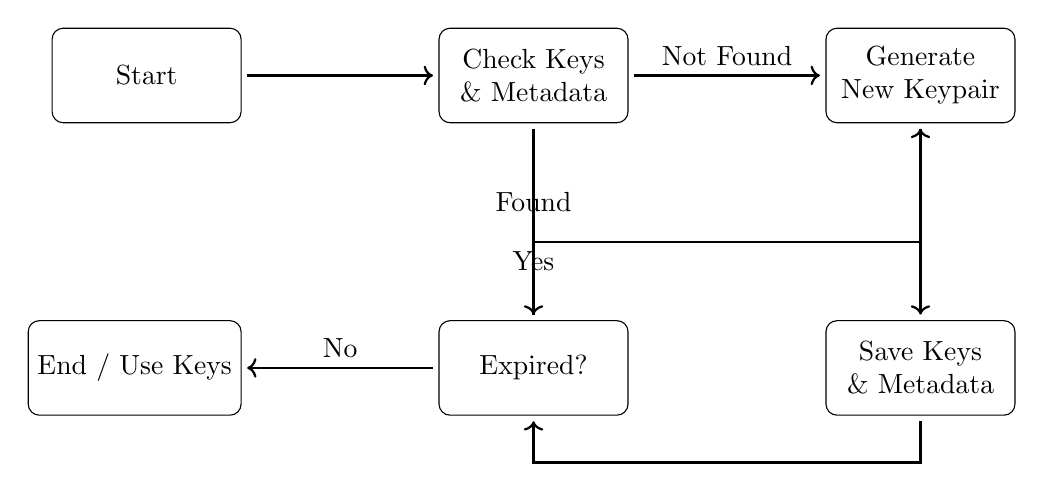
\begin{tikzpicture}[
    node distance=2.5cm, 
    box/.style={rectangle, draw, rounded corners, align=center, minimum width=2.4cm, minimum height=1.2cm},
    arrow/.style={->, thick, shorten >=2pt, shorten <=2pt}
]

% Nodes
\node[box] (start) {Start};
\node[box, right=of start] (check) {Check Keys \\ \& Metadata};
\node[box, right=of check] (generate) {Generate \\ New Keypair};
\node[box, below=of generate] (save) {Save Keys \\ \& Metadata};
\node[box, left=of save] (expire) {Expired?};
\node[box, left=of expire] (end) {End / Use Keys};

% Arrows
\draw[arrow] (start) -- (check);
\draw[arrow] (check) -- node[above]{Not Found} (generate);
\draw[arrow] (check) -- node[above]{Found} (expire);
\draw[arrow] (generate) -- (save);
\draw[arrow] (save) -- ++(0,-1.2) -| (expire);
\draw[arrow] (expire) -- node[above]{Yes} ++(0,1.6) -| (generate);
\draw[arrow] (expire) -- node[above]{No} (end);

\end{tikzpicture}
\caption{Key Management Workflow}
\label{fig:key_management_workflow}
\end{figure}

In Figure~\ref{fig:key_management_workflow}:
\begin{enumerate}
    \item The system begins by checking whether key files and metadata exist.
    \item If missing, new keys are created and saved.
    \item If present, the system evaluates whether the keys have expired.
    \item If expired, the keys are regenerated and saved (rotated).
    \item Otherwise, the keys are ready for normal usage.
\end{enumerate}

% -------------------------------------------------------------------
% 3. SECURITY ANALYSIS
% -------------------------------------------------------------------
\section{Security Analysis}

\subsection{Naive Factoring of Small RSA Moduli}
\subsubsection{Principle}
One component of the security analysis is to demonstrate the ease of factoring \emph{small} RSA moduli. An RSA modulus \(n\) is simply the product of two primes \(p\) and \(q\). If the key size is extremely small (e.g., 32 or 48 bits total), a brute-force or naive approach that attempts dividing \(n\) by candidate factors up to \(\sqrt{n}\) will succeed quickly.

\subsubsection{Method}
\begin{itemize}
    \item \textbf{Enumerate possible factors:} Start from 3 and increment in steps of 2 (skipping even numbers), testing for divisibility of \(n\).
    \item \textbf{Stop at \(\sqrt{n}\):} If \(p\) is a prime factor, it cannot exceed \(\sqrt{n}\). Thus, searching beyond \(\sqrt{n}\) is unnecessary.
\end{itemize}

\subsubsection{Correctness}
The method is grounded in the fundamental property of integer factorization:
\[
    \text{If }n = p \cdot q,\text{ then } p \le \sqrt{n}.
\]
Hence, it \emph{must} find the factors if \(n\) is small enough. For large \(n\) (e.g., 2048 bits), this approach is computationally infeasible. The demonstration proves \emph{why} cryptographic best practices require large key sizes.

\subsection{Timing Attack Demonstration}
\subsubsection{Principle}
A \emph{timing attack} attempts to deduce private information by measuring how long an operation (e.g., RSA decryption) takes under various conditions. If an implementation is not \emph{constant-time}, different parts of the algorithm might take slightly different amounts of time, revealing subtle clues about the key.

\subsubsection{Method}
\begin{itemize}
    \item \textbf{Encrypt a set of sample messages:} The system creates ciphertexts for different plaintexts.
    \item \textbf{Measure decryption time repeatedly:} Each ciphertext is decrypted multiple times, and the elapsed time is recorded.
    \item \textbf{Analyze differences:} By comparing the average and standard deviation of decryption times, one can see if certain ciphertexts yield longer or shorter durations, which might indicate how the algorithm branches internally.
\end{itemize}

\subsubsection{Correctness}
Although \emph{timing attacks} rely on statistical patterns, the demonstration code repeatedly decrypts test ciphertexts to capture average and variance in runtime. Correctness is validated by:
\begin{itemize}
    \item Repeated measurements, reducing random noise.
    \item Aggregating results across multiple ciphertexts to highlight potential differences.
\end{itemize}
In a real-world scenario, truly constant-time cryptographic implementations mitigate or eliminate these observable patterns.

\subsection{Conceptual Diagram of Factoring and Timing Workflows}
\begin{figure}[h!]
\centering
\resizebox{\textwidth}{!}{%
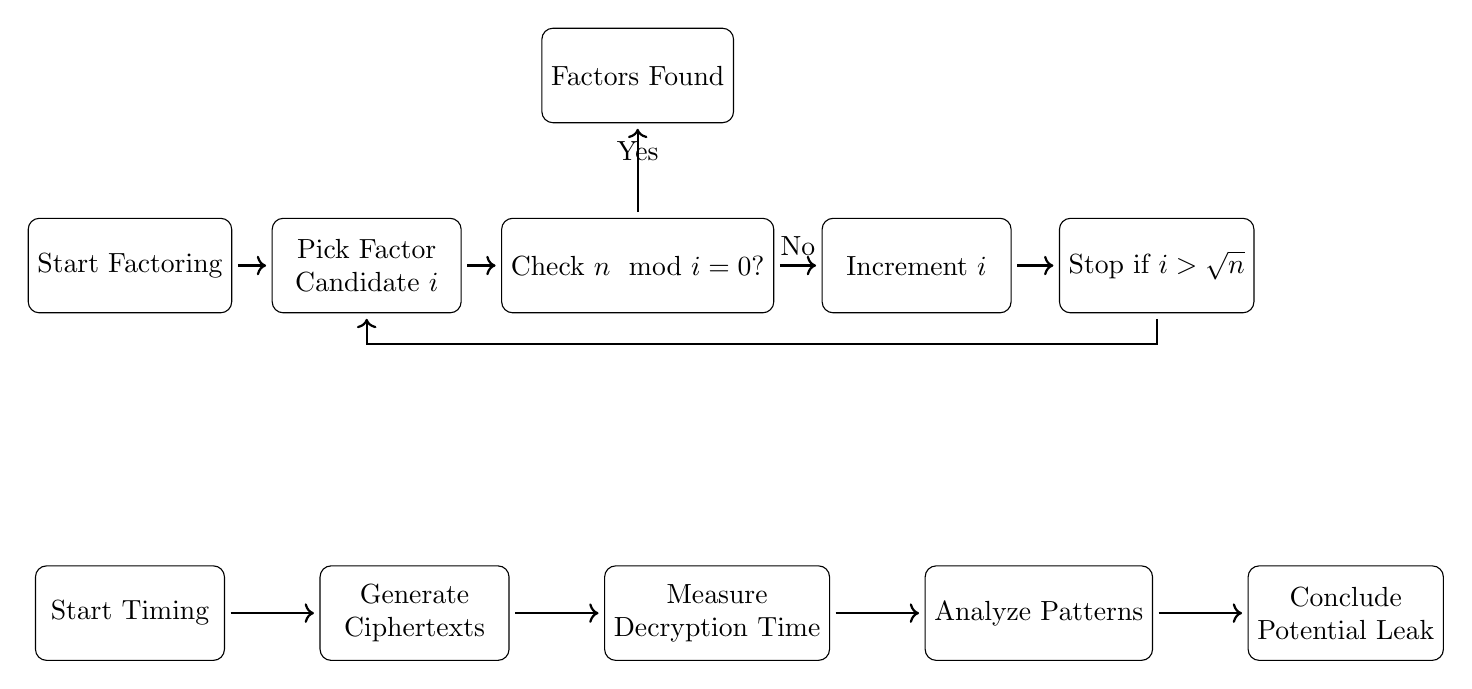
\begin{tikzpicture}[
    node distance=2cm,
    box/.style={rectangle, draw, rounded corners, align=center, 
                minimum width=2.4cm, minimum height=1.2cm},
    arrow/.style={->, thick, shorten >=2pt, shorten <=2pt}
]

% Factoring part
\node[box] (startF) {Start Factoring};
\node[box, right=0.5 of startF] (candidate) {Pick Factor \\ Candidate $i$};
\node[box, right=0.5 of candidate] (check) {Check $n \mod i = 0$?};
\node[box, above=1.2 of check] (found) {Factors Found};
\node[box, right=0.6 of check] (no) {Increment $i$};
\node[box, right=0.6 of no] (stop) {Stop if $i > \sqrt{n}$};

\draw[arrow] (startF) -- (candidate);
\draw[arrow] (candidate) -- (check);
\draw[arrow] (check) -- node[above]{Yes} (found);
\draw[arrow] (check) -- node[above]{No} (no);
\draw[arrow] (no) -- (stop);
\draw[arrow] (stop) -- ++(0,-1) -| (candidate);

% Timing attack part
\node[box, below=3.2 of startF] (startT) {Start Timing};
\node[box, right=1.2 of startT] (encrypt) {Generate \\ Ciphertexts};
\node[box, right=1.2 of encrypt] (measure) {Measure \\ Decryption Time};
\node[box, right=1.2 of measure] (analyze) {Analyze Patterns};
\node[box, right=1.2 of analyze] (conclude) {Conclude \\ Potential Leak};

\draw[arrow] (startT) -- (encrypt);
\draw[arrow] (encrypt) -- (measure);
\draw[arrow] (measure) -- (analyze);
\draw[arrow] (analyze) -- (conclude);

\end{tikzpicture}
} % end of \resizebox
\caption{High-level Workflows for Naive Factoring and Timing Analysis}
\label{fig:factoring_timing_diagram}
\end{figure}


% -------------------------------------------------------------------
% 4. CONCLUSION
% -------------------------------------------------------------------
\section{Conclusion}

In summary, this project illustrates:
\begin{itemize}
    \item A robust \textbf{key management} lifecycle, with metadata-driven key generation, expiration checks, and automatic rotation.
    \item The \textbf{vulnerability} of small RSA keys to naive factoring, emphasizing the need for key sizes of at least 2048 bits for practical security.
    \item A \textbf{timing attack} demonstration that reveals how measuring decryption times can potentially leak sensitive information when cryptographic operations are not constant-time.
\end{itemize}

\noindent
\textbf{Future enhancements} could include:
\begin{itemize}
    \item More rigorous integration with a secure keystore or hardware security module (HSM).
    \item Tools for rotating keys based on usage thresholds (not just a time-based expiration).
    \item Countermeasures for timing attacks (constant-time modular exponentiation, blinding techniques, etc.).
\end{itemize}

\end{document}
